%\documentclass[twoside]{report}
\documentclass[12pt]{article}
\usepackage{ecj,palatino,epsfig,latexsym,natbib}
\usepackage{enumitem}
\usepackage{amsmath, amsthm, amssymb}
\usepackage{graphicx}
\usepackage{siunitx} % Required for alignment


\usepackage{sectsty}
\usepackage[dvipsnames]{xcolor}
\sectionfont{\color{cyan}}  % sets colour of chapters
\subsectionfont{\color{blue}} 
\sisetup{
  round-mode          = places, % Rounds numbers
  round-precision     = 3, % to 2 places
}

\newcommand\tab[1][1cm]{\hspace*{#1}}
%% do not add any other page- or text-size instruction here

\parskip=0.5 cm

\begin{document}


\title{\bf POS Tagging-Assignment II} 

\author{\name{\bf Arkajyoti Pal} \hfill \addr{arkapal.pal@gmail.com}\\ 
        \addr{\bf 15CS30003}
}

\maketitle



\section{Generative vs. Discriminative Models}
\begin{itemize}
    \item \textbf{Neural Networks}: \textit{Discriminative}. Intuitively, neural networks can be seen as a combination of \textit{perceptrons} which themselves are discriminative. Also, the likelihood and log-likelihood objective functions in a neural network are both equivalent to the probability distribution $P(Y|X)$ as:  $L(\theta)=L(\theta;X,Y)=P(Y|X,\theta)$.
    \item \textbf{Naive Bayes classifier}: \textit{Generative}. This is because it explicitly models the joint probability distribution $P(X,Y)$ and then uses the Bayes rule to compute $P(Y|X)$.
    \item \textbf{Logistice Regression}: \textit{Discriminative}. This is because it essentially models the conditional $P(Y|X)$ as a function of the input of variables and then estimates the parameters of this function from the training data. 
    \item \textbf{Gaussian Mixture model}: \textit{Generative}. It explicitly tries to explicitly model the joint distribution $P(X|Y)$ as $P(Y)P(X|Y)$ by assuming that the data points are generated as first sampling a cluster($P(Y)$) and then, given the cluster,  a data point from a Gaussian distribution around that cluster center is drawn($P(X|Y)$).
    \item \textbf{GANs}: \textit{Generative Model}. GANs try to estimate the joint distribution $P(X,Y)$ by training a generator and a discriminator in an adversarial fashion.
    \item \textbf{Latent Dirichlet Allocation}: \textit{Generative}. LDA is a generative probabilistic model of a corpus, wherein the documents are represented as random mixtures over latent topics and a topic is characterized by a distribution over words.
    \item \textbf{SVM}: SVM is a \textit{Discriminative} model that learns the optimal separating hyperplane given training data and hence tries to model the conditional distribution $P(Y|X)$.
    \item \textbf{Decision Trees}: \textit{Discriminative}. This is because they model the dependence of unobserved (target) variables $y$ on observed variables $x$. 
\end{itemize}


\section{POS Tagging with Hidden Markov Model}

\subsection{HMM}
Hidden Markov Model is a stochastic model in which the system being modeled is assumed to
be a Markov Process with latent states and observable outputs. Hidden Markov Model
consists of three components:
\begin{itemize}
 \item \textbf{$\pi(S_i)$}:Probability of the system starting in state $S_i$.
\item \textbf{$P_T(S_j|S_i)$}: Probability of the system transitioning from state $S_i$
 to state $S_j$.
\item \textbf{$P_E(Y_j|S_i)$}:Probability of the system emitting output  $Y_j$	
 in state $S_i$.
 \end{itemize}
In the specific case of our Part of Speech Tagger, the set of 12 tags(\{'DET', 'NOUN', 'ADJ', 'VERB', 'ADP', '.', 'ADV', 'CONJ', 'PRT', 'PRON', 'NUM', 'X'\}) in addition to the end-of-sentence marker '$<$/s$>$' as the end(final) state  are assumed to be the states and the
words are assumed to be the outputs. Hence, our Part of Speech Tagger consists of:
\begin{itemize}
 \item \textbf{$\pi(T_i)$}:Probability of the sequence starting in tag $T_i$.
\item \textbf{$P_T(S_j|S_i)$}:Probability of the sequence transitioning from tag $T_i$.
 to tag	$T_j$.
\item \textbf{$P_E(W_j|T_i)$}: Probability of the sequence emitting word  $W_j$	
 on tag $T_i$.
  \end{itemize}
  
 Since the number of states(tags) is not large, smoothing was not found necessary for transition or start-state probabilities. However, to account for OOV words in emission probabilities additive smoothing was implemented as:
 \begin{equation}
     \begin{split}
         P_E(w_j|t_i)=\frac{C(q_l=t_i,o_l=w_j)+\delta}{C(q_l=t_)+\delta *m},\: where\:1\leq  j \leq m \:and\\ \:m\: is \:the\: distinct \:number\: of \:words \:in \:the \:corpus.
         \\ \delta=0.001.
     \end{split}
 \end{equation}
 \subsection{Evaluating Performance}

\begin{table}[h!]
\begin{center}
    \caption{Performance of HMM Tagger}
    \label{tab:table1}
\begin{tabular}{ c c c c c}
 \textbf{Tags}& \textbf{Precision} & \textbf{Recall} & \textbf{F1-score} & \textbf{Support} \\ 
 \hline
 .  &   0.977  &   0.997  &   0.987  &     334\\  
ADJ &    0.804  &   0.879  &   0.840   &    140\\
ADP &     0.951  &   0.958  &   0.954  &     283\\
ADV  &    0.797  &   0.823  &   0.810  &     124\\
CONJ &     0.913  &   1.000 &    0.955  &      84\\
DET  &    0.977  &   0.990  &   0.983   &    295\\
NOUN &     0.953 &    0.849 &    0.898  &     483\\
NUM  &    0.455  &   0.952  &   0.615  &      21\\
PRON  &    0.958 &    0.994 &    0.975  &     160\\
PRT  &    0.890  &   0.929  &   0.909   &     70\\
VERB &     0.962 &    0.884 &    0.921  &     370\\
X   &   0.367   &  0.647    &    0.468    &    17\\
\hline
\textbf{avg / total}  &     0.932&      0.923 &     0.925  &     2381

\end{tabular}
\end{center}
\end{table}
As we can see from Table \ref{tab:table1}, the overall(weighted) F1-score comes out to be \textbf{92.5\%}.

\section{POS Tagging with Conditional Random Fields}

To justify the inclusion of a feature in the feature set of the CRF-based POS Tagger, we first introduce a 'baseline' model with only the current word and bias term as the baseline features. Subsequently, we justify the inclusion of the features proposed with an intuitive explanation and also show their improvement over the baseline scores.

\subsection{Baseline Model}

\textbf{\textit{Features}}:The baseline features include a bias term and the current word. Table \ref{tab:table2} shows the performance of the baseline model.

\begin{table}[h!]
\begin{center}
    \caption{Performance of Baseline CRF Model}
    \label{tab:table2}
\begin{tabular}{ c c c c c}
 \textbf{Tags}& \textbf{Precision} & \textbf{Recall} & \textbf{F1-score} & \textbf{Support} \\ 
 \hline
          .  &     1.000   &   1.000  &    1.000   &     334\\
          X   &    0.000   &   0.000  &    0.000   &      17\\
        ADJ   &    0.827   &   0.786   &   0.806   &     140\\
        ADP  &     0.962   &   0.972   &   0.967    &    283\\
        ADV   &    0.902  &    0.815  &    0.856    &    124\\
       VERB  &     0.968  &    0.900  &    0.933   &     370\\
        DET  &     0.993  &    0.997  &    0.995   &     295\\
       CONJ   &    1.000  &    0.988   &   0.994   &      84\\
       NOUN   &    0.863  &    0.969   &   0.913   &    483\\
       PRON  &     0.994  &    0.981   &   0.987   &     160\\
        PRT  &     0.889  &    0.914   &   0.901   &      70\\
        NUM  &     0.952  &    0.952   &   0.952    &     21\\
\hline
\textbf{avg / total}    &    0.935   &   0.940    &  0.937     &  2381

\end{tabular}
\end{center}
\end{table}

\subsection{Previous and Next Word as a feature}
In addition to the baseline features, we propose using the  previous(if the current word is not the first word) and the next word(if the current word is not the last word) as a feature.\\
\textbf{Intuition}:
Table \ref{tab:table3} shows an improved F1-score of 94.8\% over the 93.7\% of the baseline model justifying our inclusion.
\begin{table}[h!]
\begin{center}
    \caption{Performance of CRF Model with Prefix as a Feature}
    \label{tab:table3}
\begin{tabular}{ c c c c c}
 \textbf{Tags}& \textbf{Precision} & \textbf{Recall} & \textbf{F1-score} & \textbf{Support} \\ 
 \hline

          .   &   1.000  &   1.000 &    1.000    &   334\\
          X   &   1.000  &   0.118 &    0.211    &    17\\
        ADJ   &   0.847 &    0.793 &    0.819    &   140\\
        ADP   &   0.975 &    0.979 &    0.977    &   283\\
        ADV   &   0.913 &    0.847 &    0.879    &   124\\
       VERB  &    0.966 &    0.930 &    0.948    &   370\\
        DET  &    0.993  &   1.000 &    0.997   &    295\\
       CONJ  &    1.000   &  0.976  &   0.988   &     84\\
       NOUN  &    0.886  &   0.969 &    0.926   &    483\\
       PRON   &   1.000 &    0.981 &    0.991   &    160\\
        PRT   &   0.904 &    0.943 &    0.923   &     70\\
        NUM   &   0.955  &   1.000 &    0.977   &     21\\
\hline
\textbf{avg / total}&      0.951 &    0.950  &   0.948  &    2381
 
 \end{tabular}
\end{center}
\end{table}


\subsection{Prefix of different lengths as a feature}
In addition to the baseline features, we propose using the prefixes of length 2 and 3 of the current, previous(if the current word is not the first word) and the next word(if the current word is not the last word) as a feature.\\
\textbf{Intuition}:

Table \ref{tab:table4} shows an improved F1-score of 94.94\% over the 93.7\% of the baseline model justifying our inclusion.
\begin{table}[h!]
\begin{center}
    \caption{Performance of CRF Model with Prefix as a Feature}
    \label{tab:table4}
\begin{tabular}{ c c c c c}
 \textbf{Tags}& \textbf{Precision} & \textbf{Recall} & \textbf{F1-score} & \textbf{Support} \\ 
 \hline

          .   &   1.000  &  1.000  &   1.000   &       334\\ 
          X   &   1.000  &   0.294  &   0.455  &      17\\ 
        ADJ   &   0.839  &   0.821  &   0.830  &     140\\ 
        ADP   &   0.969  &   0.979  &   0.974  &     283\\ 
        ADV   &   0.927  &   0.815  &   0.867  &     124\\ 
       VERB   &   0.958  &   0.930  &   0.944  &     370\\ 
        DET   &   0.993  &   1.000  &   0.997  &     295\\ 
       CONJ   &   1.000  &   0.976  &   0.988  &      84\\ 
       NOUN   &   0.901  &   0.965  &   0.932  &     483\\ 
       PRON   &   0.994   &  0.994  &   0.994  &     160\\ 
        PRT   &   0.892  &   0.943  &   0.917  &      70\\ 
        NUM    &  0.952 &    0.952  &   0.952  &      21\\ 
\hline
\textbf{avg / total} &     0.952 &    0.951 &     0.949  &    2381

\end{tabular}
\end{center}
\end{table}


\subsection{Suffix of different lengths as a feature}

In addition to the baseline features, we propose using the suffixes of length 2 and 3 of the current, previous(if the current word is not the first word) and the next word(if the current word is not the last word) as a feature.\\
\textbf{Intuition}:

Table \ref{tab:table5} shows an improved F1-score of 95.57\% over the 93.7\% of the baseline model justifying our inclusion.


\begin{table}[h!]
\begin{center}
    \caption{Performance of CRF Model with Suffix as a Feature}
    \label{tab:table5}
\begin{tabular}{ c c c c c}
 \textbf{Tags}& \textbf{Precision} & \textbf{Recall} & \textbf{F1-score} & \textbf{Support} \\ 
 \hline


          .  &    1.000 &    1.000 &    1.000    &   334\\ 
          X   &   1.000  &   0.176 &    0.300    &    17\\ 
        ADJ   &   0.830  &   0.836 &    0.833    &   140\\ 
        ADP  &    0.968  &   0.975 &    0.972    &   283\\ 
        ADV  &    0.932  &   0.879 &    0.905    &   124\\ 
       VERB  &    0.970  &   0.946 &    0.958    &   370\\
        DET  &    0.997  &   0.997 &    0.997    &   295\\ 
       CONJ  &    1.000  &   0.976 &    0.988    &    84\\ 
       NOUN  &    0.923  &   0.971 &    0.947    &   483\\ 
       PRON  &    0.994  &   0.988 &    0.991    &   160\\ 
        PRT  &    0.893  &   0.957 &    0.924    &    70\\ 
        NUM  &    1.000  &   1.000 &    1.000    &    21\\ 
\hline
\textbf{avg / total} &   0.958  &   0.958  &   0.956   &   2381

\end{tabular}
\end{center}
\end{table}

\subsection{Additional Boolean Features}
In addition to the baseline and above mentioned features, we propose using three boolean features; namely:
\begin{itemize}
    \item The Word is a title. For example: Palantir.
    \item All the letters in the word are upper cased.
    \item The string is numeric.
    
\end{itemize}
of the current, previous(if the current word is not the first word) and the next word(if the current word is not the last word) as a feature.\\
\textbf{Intuition}:
Table \ref{tab:table6} shows an improved F1-score of 94.28\% over the 93.7\% of the baseline model justifying our inclusion.
\begin{table}[h!]
\begin{center}
    \caption{Performance of CRF Model with Suffix as a Feature}
    \label{tab:table6}
\begin{tabular}{ c c c c c}
 \textbf{Tags}& \textbf{Precision} & \textbf{Recall} & \textbf{F1-score} & \textbf{Support} \\ 
 \hline

          .   &   1.000  &   1.000  &   1.000  &     334\\ 
          X   &   0.000  &   0.000  &   0.000  &      17\\ 
        ADJ   &   0.830  &   0.800  &   0.815  &     140\\ 
        ADP   &   0.975  &   0.975  &   0.975  &     283\\ 
        ADV   &   0.913  &   0.847  &   0.879  &     124\\ 
       VERB   &   0.961  &   0.924  &   0.942  &     370\\ 
        DET   &   0.993  &   1.000  &   0.997  &     295\\ 
       CONJ   &   1.000  &   0.976  &   0.988  &      84\\ 
       NOUN  &    0.881  &   0.963  &   0.920  &     483\\ 
       PRON  &    1.000  &   0.981  &   0.991  &     160\\ 
        PRT  &    0.892  &   0.943  &   0.917  &      70\\ 
        NUM  &    0.950  &   0.905  &   0.927  &      21\\ 
\hline
\textbf{avg / total} &    0.941  &   0.946     0.943   &   2381

\end{tabular}
\end{center}
\end{table}

\subsection{Final Model}
We include all the above mentioned features in our feature set. Additionally, we also include two indicator variables to denote if the current word is the start or the end of the current sentence.
With the given coefficients of \textit{L1} and \textit{L2 Regularization} as 0.1, as Table \ref{tab:table7} shows, an F1-score of \textbf{95.82\%} is achieved which is a considerable improvement over  the HMM model.\\
However, we show in the following section that tuning the hyperparamters improves the F1-score even further.

\begin{table}[h!]
\begin{center}
    \caption{Performance of the CRF Model with all the mentioned features}
    \label{tab:table7}
\begin{tabular}{ c c c c c}
 \textbf{Tags}& \textbf{Precision} & \textbf{Recall} & \textbf{F1-score} & \textbf{Support} \\ 
 \hline

          .  &     1.000   &   1.000 &     1.000  &      334\\
          X   &    1.000    &  0.176 &     0.300  &       17\\
        ADJ &      0.861    &  0.886 &     0.873  &      140\\
        ADP   &    0.968   &    0.975 &     0.972 &      283\\
        ADV &      0.924  &    0.879  &    0.901   &     124\\
       VERB   &    0.975    &  0.938  &    0.956   &      370\\
        DET &      0.997    &  1.000 &     0.998  &      295\\
       CONJ   &    1.000     & 0.976 &     0.988  &       84\\
       NOUN &      0.927    &  0.967 &     0.946  &      483\\
       PRON   &    1.000  &    1.000 &     1.000 &       160\\
        PRT &      0.883    &  0.971 &     0.925 &        70\\
        NUM   &    0.955  &    1.000  &    0.977  &       21\\
\hline
\textbf{avg / total} &      0.961   &   0.960  &    0.958 &      2381

\end{tabular}
\end{center}
\end{table}

\subsection{Hyperparameter Optimization}
For choosing hyperparameters, we perform a randomized search with 3-fold cross validation. The coefficients for \textit{L1} and \textit{L2} Regularization are sampled from an exponential distribution with scale 0.5 and 0.05 respectively.
The results corresponding to each pair sampled can be seen from the ipynb notebook while Fig.\ref{fig:plot1} shows the points that have been sampled: blue signifies poorer performance while red shades signify better results.\\
\\
The best parameters returned by the search were:\\
c1(L1 Regularization Coefficient): 0.3750756963753804, \\c2(L2 Regularization Coefficient): 0.004186602148178022.\\
\\
The performance of the CRF Model with the above coefficients has been enumerated in Table \ref{tab:table8} which shows an F1-score of \textsc{\textbf{96.1\%}}, a considerable improvement over the previous model(without parameter search).
\begin{figure}[h!]
  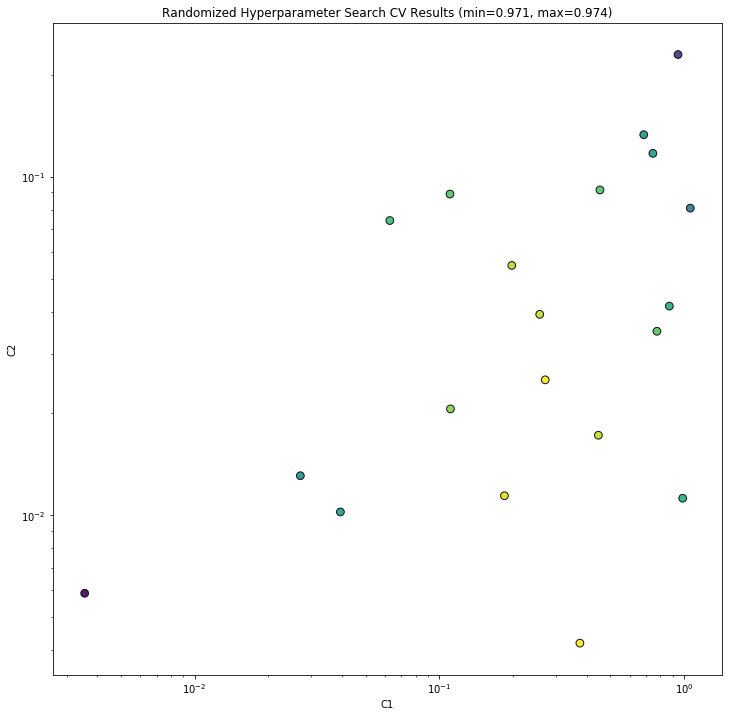
\includegraphics[width=10 cm]{plot.png}
  \caption{Sampled Regularization Coefficients. Dark blue= 0.9709, dark red = 0.9737}
  \label{fig:plot1}
\end{figure}

\begin{table}[h!]
\begin{center}
    \caption{Performance of hyperparameter tuned CRF Model}
    \label{tab:table8}
\begin{tabular}{ c c c c c}
 \textbf{Tags}& \textbf{Precision} & \textbf{Recall} & \textbf{F1-score} & \textbf{Support} \\ 
 \hline

          .   &    1.000 &     1.000  &    1.000  &      334\\ 
          X &      0.875 &     0.412  &    0.560  &       17\\ 
        ADJ   &    0.848 &     0.879  &    0.863  &      140\\ 
        ADP  &     0.975  &    0.979 &     0.977  &      283\\ 
        ADV  &     0.923  &    0.871 &     0.896  &      124\\ 
       VERB  &     0.969  &    0.943  &    0.956  &      370\\ 
        DET  &     0.997  &    1.000  &    0.998  &      295\\ 
       CONJ  &     1.000  &    0.976 &     0.988  &       84\\ 
       NOUN &      0.936  &    0.963 &     0.949  &      483\\ 
       PRON &      1.000  &    1.000 &     1.000  &      160\\ 
        PRT &      0.895  &    0.971 &     0.932  &       70\\ 
        NUM &      0.955  &    1.000 &     0.977  &       21\\ 
\hline
\textbf{avg / total} &    0.962 &     0.961 &      \textbf{0.961}   &    2381

\end{tabular}
\end{center}
\end{table}

\section{Conclusion}
The (hyperparameter optimized) CRF model gives much better performance on the test data as compared to the HMM based POS tagger as is expected. However, the increase in performance comes at the cost of considerably higher training time for the CRF Model as compared to the HMM.

\end{document}
